\chapter{Monte Carlo Solution Methods for the Simplified $P_N$ Equations}
\label{ch:spn_equations}

The neutron transport problem is complicated. Solutions cover a large
phase space and the problems of interest are often geometrically
complex, very large, or both, requiring tremendous computational
resources to generate an adequate solution. Modern deterministic
methods for large scale problems are commonly variants on the discrete
ordinates ($S_N$) method \citep{evans_denovo:_2010}. For full reactor
core neutronics simulations, the $S_N$ method requires potentially
trillions of unknown angular flux moments to be computed to achieve
good accuracy for the repsonses of interest
\citep{slaybaugh_acceleration_2011}. Other forms of the transport
problem, including the $P_N$ method, take on a simpler form than the
more common $S_N$ methods but lack in accuracy when compared while
still requiring considerable computational resources for solutions in
multiple dimensions.

In the 1960's, Gelbard developed an ad-hoc multidimensional extension
of the simple single dimension planar $P_N$ equations that created a
system of coupled, diffusion-like equations known as the simplified
$P_N$ ($SP_N$) equations. Up until around the 1990's, the $SP_N$
method was either widely unknown, widely unused, or combination of
both even though numerical studies showed promising results with
better solutions than diffusion theory and a significant reduction in
computational time over more accurate methods such as discrete
ordinates. Why did this happen? A significant problem, pointed out by
Brantley and Larsen \citep{brantley_simplified_2000}, was that little
rigor had been applied to the formulation of the $SP_N$ equations
since their derivation through primarily heuristic arguments. Instead,
studies at that time focused on simply comparing the results of the
method to other contemporary transport solution strategies. In
addition, many problems of interest from the literature at the time
were either solved using nodal-type methods for reactor-sized problems
or $S_N$-type methods for benchmark problems with intricate material
configurations and potentially large flux gradients over small spatial
domains.

So why reconsider the $SP_N$ equations? Starting in the 1990's and
primarily due to Larsen and his colleagues, the $SP_N$ equations have
been given a more rigorous treatment with both variational and
asymptotic derivations performed as a means of verification. In
addition, these equations have been more rigorously studied as
solution methods to MOX fuel problems and have been shown to provide
accurate solutions. With this mathematical literature to provide a
solid numerical footing for the method, we look at its application to
today's challenge problems in full reactor core transport. The
reduction in numerical complexity of current full core deterministic
solution methods using the $S_N$ approximation could mean significant
savings in both compute time and memory required. In addition, the
characteristics of the solution to the transport problem for a steady
state reactor core permit diffusion theory to be used; a staple of the
nuclear industry since its inception. Therefore, if diffusion theory
is applicable, then finer grained solutions that capture more of the
physics contained in the transport equation should be possible with
the $SP_N$ method. In doing so, we also expect from the literature to
obtain computed responses on the order of accuracy we would expect
from an appropriately discretized $S_N$ method at a fraction of the
cost. 

To further motivate moving in this direction, recent developments in
the Exnihilo neutronics package at Oak Ridge National Laboratory have
permitted generation of the $SP_N$ system of equations for detailed
full core reactor models \citep{evans_simpli_2013}. By fully forming
these equations and formulating them as a linear algebra problem
instead of using the explicit iterative methods of the past, we now
have access to all of the modern advancements in computational linear
algebra including Krylov solvers for asymmetric systems and
preconditioning methods such as algebraic multigrid. This leads us to
then explore the applicability of our work in discrete Monte Carlo
methods for linear systems as a possible solution method for the
$SP_N$ equations. If formulated correctly, we hypothesize that
signficant improvement in usage of computational resources may be
observed compared to modern solution techniques such as those
suggested due to the form of the matrices generated by the
discretization. In addition, solving the $SP_N$ equations in this way
also breaks away from the $S_N$ forms of parallelism where spatial
parallelism is achieved by an efficient parallel sweep, angular
efficiency achieved by pipelining, and energy parallelism achieved by
decoupling the groups. With the $SP_N$ equations as a full matrix
system, we now can parallelize the problem as prescribed by the linear
solver, which may be significantly more scalable than current $S_N$
transport practices.

In this chapter, we derive the $SP_N$ equations, closely following the
work of Evans, in order to gain full understanding of the underlying
system and its potential behavior in a Monte Carlo context. From the
$P_N$ equations, we apply a set of approximations to yield the
multi-dimensional, multi-group $SP_N$ equations for fixed source
problems\footnote{The $SP_N$ derivations in this chapter are heavily
  based on those presented by Evans in
  \citep{evans_simpli_2013}}. Using the fully-formed matrix for the
transport problem, we explore solutions to the $SP_N$ equations using
Monte Carlo Synthetic Acceleration using a light water reactor fuel
assembly criticality calculation as the driving problem.

%%---------------------------------------------------------------------------%%
\section{The Neutron Transport Equation}
\label{sec:transport_eq}
As a starting point we define the time-independent neutron transport
equation \citep{lewis_computational_1993}:
\begin{multline}
  \hat{\Omega} \cdot \vec{\nabla} \psi(\vec{r},\hat{\Omega},E) +
  \sigma(\vec{r},E) \psi(\vec{r},\hat{\Omega},E) = \\ \int \int
  \sigma_s(\vec{r},E' \rightarrow E,\hat{\Omega}' \rightarrow
  \hat{\Omega}) \psi(\vec{r},\hat{\Omega}',E') d\Omega' dE' +
  q(\vec{r},\hat{\Omega},E)\:,
  \label{eq:general_transport}
\end{multline}
with the variables defined as:
\begin{itemize}
\item $\vec{r}$ - neutron spatial position
\item $\hat{\Omega}$ - neutron streaming direction with radial
  component $\mu$ and azimuthal component $\omega$
\item $\hat{\Omega}' \cdot \hat{\Omega} = \mu_0$ is the angle of
  scattering
\item $E$ - neutron energy
\item $\psi(\vec{r},\hat{\Omega},E)$ - angular flux
\item $\sigma(\vec{r},E)$ - total interaction cross section
\item $\sigma_s(\vec{r},E' \rightarrow E,\hat{\Omega}')$ - probability
  of scattering from direction $\hat{\Omega}'$ into an angular domain
  $d\hat{\Omega}'$ about the direction $\hat{\Omega}$ and from energy
  $E'$ to an energy domain $dE'$ about energy $E$
\item $q(\vec{r},\hat{\Omega},E)$ - external source of neutrons.
\end{itemize}
For this work, it is sufficient to formulate
Eq~(\ref{eq:general_transport}) in 1-dimensonal Cartesian geometry:
\begin{multline}
  \mu \frac{\partial}{\partial x} \psi(x,\mu,E) + \sigma(x,E)
  \psi(x,\mu,E) = \\ \int \int \sigma_s(x,E') \rightarrow
  E,\hat{\Omega}' \rightarrow \hat{\Omega}) \psi(x,\hat{\Omega}',E')
  d\Omega' dE' + \frac{q(x,E)}{4 \pi}\:,
  \label{eq:cart_1d_transport}
\end{multline}
where the angular component of the solution is no longer dependent on
the azimuthal direction of travel and an isotropic source of neutrons
is assumed.

%%---------------------------------------------------------------------------%%
\section{Derivation of the Monoenergetic $SP_N$ Equations}
\label{sec:spn_equations}
The $P_N$ equations as derived in Appendix~\ref{chap:pn_equations}
give $N+1$ coupled first-order equations capturing the spatial and
angular-dependence of the solution. In multiple dimensions, the
equation set becomes large and coupled not only through angular
moments but also through the spatial variables. As a simpler
alternative to multidimensional $P_N$ solutions, Gelbard recognized in
1960 that the planar $P_N$ equations could be simplified and applied
an ad-hoc method to extend them to multiple dimensions, yielding the
$SP_N$ equations. These equations are not only fewer in number, but
also take on a diffusion-like form while maintaining the angular
character of the flux, making them amenable to solutions with modern
diffusion methods.

First, the $P_N$ equations can be simplified to $(N+1)/2$ second-order
equations by solving for the $n^{th}$ Legendre flux moment in the
odd-order equations:
\begin{equation}
  \phi_n = \frac{1}{\Sigma_n}\Bigg[ q \delta_{no} -
    \frac{\partial}{\partial x}\Big(\frac{n}{2n+1}\phi_{n-1} +
    \frac{n+1}{2n+1} \phi_{n+1} \Big) \Bigg]\:, 
  \label{eq:odd_moments}
\end{equation}
for $n = 1,3,\cdots,N$ and $\delta_{no} = 0\ \forall n \neq 0$. We can
insert the odd moments into Eq~(\ref{eq:final_pn_equations}) to get a
reduced group of equations for the even moments:
\begin{multline}
  -\frac{\partial}{\partial x}
  \Bigg[\frac{n}{2n+1}\frac{1}{\Sigma_{n-1}} \frac{\partial}{\partial
      x} \Big(\frac{n-1}{2n-1} \phi_{n-2} + \frac{n}{2n-1}\phi_n \Big)
    \\+ \frac{n+1}{2n+1}\frac{1}{\Sigma_{n+1}} \frac{\partial}{\partial
      x} \Big(\frac{n+1}{2n+3}\phi_n + \frac{n+2}{2n+3}\phi_{n+2}\Big)
    \Bigg] \\+ \Sigma_n \phi_n = q \delta_{n0}\ \ \ \ \ \ \ \ \ n =
  0,2,4,\cdots,N\:.
  \label{eq:reduced_pn}
\end{multline}
Immediately, we note the diffusion-like nature of
Eq~(\ref{eq:reduced_pn}) as compared to the original $P_N$
equations. To extend these equations to multiple dimensions, Gelbard
simply replaced the planar spatial derivatives in the reduced set of
equations with general multidimensional gradient operators:
\begin{multline}
  -\nabla \cdot \Bigg[\frac{n}{2n+1}\frac{1}{\Sigma_{n-1}} \nabla
    \Big(\frac{n-1}{2n-1} \phi_{n-2} + \frac{n}{2n-1}\phi_n \Big) \\+
    \frac{n+1}{2n+1}\frac{1}{\Sigma_{n+1}} \nabla
    \Big(\frac{n+1}{2n+3}\phi_n + \frac{n+2}{2n+3}\phi_{n+2}\Big)
    \Bigg] \\+ \Sigma_n \phi_n = q \delta_{n0}\ \ \ \ \ \ \ \ \ n =
  0,2,4,\cdots,N\:,
  \label{eq:spn_equations}
\end{multline}
yielding a multidimensional set of $(N+1)/1$ angular coupled equations
defined as the $SP_N$ equations. As with the $P_N$ equations, we
provide closure to this set of equations with $\phi_{N+1} = 0$. As a
concrete example, we will consider the $SP_7$ equations:
\begin{subequations}
  \begin{gather}
    -\nabla \cdot \frac{1}{3 \Sigma_1} \nabla ( \phi_0 + 2\phi_2 ) +
    \Sigma_0 \phi_0 = q \\ 
    -\nabla \cdot \Bigg[ \frac{2}{15 \Sigma_1} \nabla ( \phi_0 + 2\phi_2
      ) + \frac{3}{35 \Sigma_3}\nabla( 3\phi_2 + 4\phi_4)\Bigg] +
    \Sigma_2 \phi_2 = 0\\
    -\nabla \cdot \Bigg[ \frac{4}{63 \Sigma_3} \nabla ( 3\phi_2 +
      4\phi_4 ) + \frac{5}{99 \Sigma_5}\nabla( 5\phi_4 +
      6\phi_6)\Bigg] + \Sigma_4 \phi_4 = 0\\
    -\nabla \cdot \Bigg[ \frac{6}{143 \Sigma_5} \nabla ( 5\phi_4 +
      6\phi_6 ) + \frac{7}{195 \Sigma_7}\nabla(7\phi_6)\Bigg] +
    \Sigma_6 \phi_6 = 0 \:.
  \end{gather}
  \label{eq:sp7_equations}
\end{subequations}
To further modify these equations, we can use a change of variables to
create a new group of equations such that the gradients are operating
on a single vector:
\begin{subequations}
  \begin{gather}
    u_1 = \phi_0 + 2\phi_2 \\
    u_2 = 3\phi_2 + 4\phi_4 \\
    u_3 = 5\phi_4 + 6\phi_6 \\
    u_4 = 7\phi_6 \:,
  \end{gather}
  \label{eq:spn7_subs}
\end{subequations}
or equivalently:
\begin{subequations}
  \begin{gather}
    \phi_0 = u_1 - \frac{2}{3}u_2 + \frac{8}{15}u_3 -
    \frac{16}{35}u_4 \\
    \phi_2 = \frac{1}{3}u_2 - \frac{4}{15}u_3 + \frac{8}{35}u_4\\ 
    \phi_4 = \frac{1}{5}u_3 - \frac{6}{35}u_4\\
    \phi_6 = \frac{1}{7}u_4\:.
  \end{gather}
  \label{eq:spn7_subs_inverse}
\end{subequations}
When substituted into Eq~(\ref{eq:sp7_equations}), these terms give:
\begin{subequations}
  \begin{gather}
    -\nabla \cdot \frac{1}{3 \Sigma_1} \nabla u_1 + \Sigma_0 \Bigg[
    u_1 - \frac{2}{3}u_2 + \frac{8}{15}u_3 - \frac{16}{35}u_4 \Bigg]
    = -q \\
    -\nabla \cdot \Bigg[ \frac{2}{15 \Sigma_1} \nabla u_1 +
    \frac{3}{35 \Sigma_3} \nabla u_2 \Bigg] + \Sigma_2 \Bigg[
    \frac{1}{3}u_2 - \frac{4}{15}u_3 + \frac{8}{35}u_4 \Bigg] = 0 \\
    -\nabla \cdot \Bigg[ \frac{4}{63 \Sigma_3} \nabla u_2 +
    \frac{5}{99 \Sigma_5} \nabla u_3 \Bigg] + \Sigma_4 \Bigg[
    \frac{1}{5}u_3 - \frac{6}{35}u_4 \Bigg] = 0 \\ 
    -\nabla \cdot \Bigg[ \frac{6}{143 \Sigma_5} \nabla u_3 +
    \frac{7}{195 \Sigma_7} \nabla u_4 \Bigg] + \Sigma_6 \Bigg[
    \frac{1}{7}u_4 \Bigg] = 0 \:.
  \end{gather}
  \label{eq:spn7_subs_equations}
\end{subequations}
If we rearrange the Eq~(\ref{eq:spn7_subs_equations}) such that only
one divergence operation is present in each equation, we can formulate
this as a matrix system of 4 equations in the case of the $SP_7$
approximation:
\begin{equation}
  -\nabla \cdot D_n \nabla u_n + \sum_{m=1}^4 A_{nm} u_m =
  q_n\ \ \ \ \ \ \ n = 1,2,3,4\:,
  \label{eq:spn_matrix}
\end{equation}
with $\mathbf{u}$ the vector of solution variables:
\begin{equation}
  \mathbf{u} = ( u_1\ \ u_2\ \ u_3\ \ u_4 )^T \:,
  \label{eq:spn7_solution_vector}
\end{equation}
$\mathbf{D}$ the vector of effective diffusion coefficients:
\begin{equation}
  \mathbf{D} = \Bigg( \frac{1}{3\Sigma_1}\ \ \frac{1}{7\Sigma_3}\ \
  \frac{1}{11\Sigma_5}\ \ \frac{1}{15\Sigma_7} \Bigg)^T\:,
  \label{eq:spn7_diffusion_coeffs}
\end{equation}
$\mathbf{q}$ the vector of source terms where the $0^{th}$ moment
source has now been distributed through the system:
\begin{equation}
  \mathbf{q} = (
  q\ \ -\frac{2}{3}q\ \ \frac{8}{15}q\ \ -\frac{16}{35}q )^T\:,
  \label{eq:spn7_source_vector}
\end{equation}
and $\mathbf{A}$ a matrix of angular scattering terms:
% NOTE: I copied the following matrix directly out of Tom's tech note
% on the SPn equations which I am effectively following here because I
% was feeling lazy. I have verified its correctness.
\begin{equation}
  \mathbf{A} = 
  {\tiny \begin{bmatrix}
    (\Sigma_0) &
    (-\frac{2}{3}\Sigma_0) &
    (\frac{8}{15}\Sigma_0) &
    (-\frac{16}{35}\Sigma_0) \\
    %%
    &&&\\
    %%
    (-\frac{2}{3}\Sigma_0) &
    (\frac{4}{9}\Sigma_0 + \frac{5}{9}\Sigma_2) &
    (-\frac{16}{45}\Sigma_0 - \frac{4}{9}\Sigma_2) &
    (\frac{32}{105}\Sigma_0 + \frac{8}{21}\Sigma_2) \\
    %%
    &&&\\
    %%
    (\frac{8}{15}\Sigma_0) &
    (-\frac{16}{45}\Sigma_0 - \frac{4}{9}\Sigma_2) &
    (\frac{64}{225}\Sigma_0 + \frac{16}{45}\Sigma_2 + \frac{9}{25}\Sigma_4) &
    (-\frac{128}{525}\Sigma_0 - \frac{32}{105}\Sigma_2 - \frac{54}{175}\Sigma_4)
    \\ 
    %%
    &&&\\
    %%
    (-\frac{16}{35}\Sigma_0) &
    (\frac{32}{105}\Sigma_0 + \frac{8}{21}\Sigma_2) &
    (-\frac{128}{525}\Sigma_0 - \frac{32}{105}\Sigma_2 - \frac{54}{175}\Sigma_4)
    & 
    (\frac{256}{1225}\Sigma_0 + \frac{64}{245}\Sigma_2 +
    \frac{324}{1225}\Sigma_4 + \frac{13}{49}\Sigma_6)
  \end{bmatrix}}\:.
  \label{eq:A_matrix}
\end{equation}
Note that the term $\sum_{m=1}^4 A_{nm} u_m$ in
Eq~(\ref{eq:spn_matrix}) couples the moments in each equation while
the diffusive term in each equation is only for a single
'psuedo-moment' $u_n$. This completes the derivation of the $SP_7$
equations for a single energy group. As noted by Evans
\citep{evans_simpli_2013}, lower order $SP_N$ approximations can be
generated by setting higher order even moments in this system to zero
(e.g. $\phi_6 = \phi_4 = 0$ yields the $SP_3$ equations). Boundary
conditions for these equations are provided in
Appendix~\ref{chap:spn_boundary_conditions}.

%%---------------------------------------------------------------------------%%
\section{Derivation of the Multigroup $SP_N$ Equations}
\label{sec:mg_spn_equations}
Up to this point, we have formulated the $P_N$ and subsequently the
$SP_N$ equations for a single neutron energy. To expand these
equations for multiple energies, we start by stating the multigroup
neutron transport equation for a single dimension in planar geometry:
\begin{multline}
  \mu \frac{\partial}{\partial x} \psi^g(x,\mu) + \sigma^g(x)
  \psi^g(x,\mu) = \\ \sum_{g'=0}^{G} \int
  \sigma_s^{gg'}(x,\hat{\Omega}' \rightarrow \hat{\Omega})
  \psi^{g'}(x,\hat{\Omega}') d\Omega' + \frac{q^g(x)}{4 \pi}\:,
  \label{eq:cart_1d_multigroup}
\end{multline}
where $g$ denotes the group index of $0$ to $G$ groups, $G=N_g-1$, and
the integration of the scattering emission term of energy has been
replaced by a discrete summation. For scattering, $\sigma_s^{gg'}$
provides the probability of scattering at a particular angle from
group $g$ to $g'$. The result is an equation nearly identical in form
to Eq~(\ref{eq:cart_1d_transport}) where now instead of forming the
$P_N$ and $SP_N$ equations for a single energy group, we form them for
each of the energy groups with group coupling occuring through the
scattering term. The multigroup $P_N$ equations are then:
\begin{equation}
   \frac{1}{2n+1} \frac{\partial}{\partial x}\Big[ (n+1) \phi^g_{n+1}
     + n \phi^g_{n-1} \Big] +
   \sum_{g'}(\sigma^g\delta_{gg'}-\sigma^{gg'}_{sn}) \phi^g_n =
   q\delta_{n0} \:,
  \label{eq:multigroup_pn_equations}
\end{equation}
for $n = 0,1,\dotsc,N$ where the flux and scattering moments are
defined in a group. We observe that a $N_g \times N_g$ scattering
matrix is formed:
\begin{equation}
  \mathbf{\Sigma}_n =
  \sum_{g'}(\sigma^g\delta_{gg'}-\sigma^{gg'}_{sn})\:,
  \label{eq:scattering_matrix}
\end{equation}
and when expanded gives:
%% Also grabbed this matrix from Tom's tech note.
\begin{equation}
  \mathbf{\Sigma}_n =
  \begin{bmatrix}
    (\sigma^0-\sigma_{sn}^{00}) & -\sigma_{sn}^{01} & \dots &
    -\sigma_{sn}^{0G} \\ &&&\\ -\sigma_{sn}^{10} &
    (\sigma^1-\sigma_{sn}^{11}) & \dots & -\sigma_{sn}^{1G}
    \\ &&&\\ \vdots & \vdots & \ddots & \vdots
    \\ &&&\\ -\sigma_{sn}^{G0} & -\sigma_{sn}^{G1} & \dots &
    (\sigma^G-\sigma_{sn}^{GG})
  \end{bmatrix}\:.
\end{equation}
It is also useful to combine the group flux moments and sources into a
single vector for more compact notation:
\begin{equation}
  \mathbf{\Phi_n} = (\phi^0_n\ \phi^1_n\ \cdots \phi^G_n )^T\:, 
  \label{eq:group_flux_vector}
\end{equation}
\begin{equation}
  \mathbf{q} = (q^0\ q^1\ \cdots q^G )^T\:.
  \label{eq:group_source_vector}
\end{equation}
Next, we apply the $SP_N$ approximation to
Eq~(\ref{eq:multigroup_pn_equations}) in identical fashion to the
monoenergetic case. This gives:
\begin{multline}
  -\nabla \cdot \Bigg[\frac{n}{2n+1}\mathbf{\Sigma_{n-1}}^{-1} \nabla
    \Big(\frac{n-1}{2n-1} \mathbf{\Phi_{n-2}} +
    \frac{n}{2n-1}\mathbf{\Phi_n} \Big) \\+
    \frac{n+1}{2n+1}\mathbf{\Sigma_{n+1}}^{-1} \nabla
    \Big(\frac{n+1}{2n+3}\mathbf{\Phi_n} +
    \frac{n+2}{2n+3}\mathbf{\Phi_{n+2}}\Big) \Bigg] \\+
  \mathbf{\Sigma_n} \mathbf{\Phi_n} = \mathbf{q}
  \delta_{n0}\ \ \ \ \ \ \ \ \ n = 0,2,4,\cdots,N\:.
  \label{eq:multigroup_spn_equations}
\end{multline}
This adds more complexity than the monoenergetic formulation in that
all unknowns in this group of equations are now vector quantities and
scattering relationships are contained in matrices rather than a
scalar quantity. Because of this, the same sequence of variable
changes and algebra can be used to build a set of matrix equations,
this time in a block formulation:
\begin{equation}
  -\nabla \cdot \mathbb{D}_n \nabla \mathbb{U}_n + \sum_{m=1}^4
  \mathbb{A}_{nm} \mathbb{U}_m = \mathbb{Q}_n\:,
  \label{eq:spn_multigroup_system}
\end{equation}
where the definition of all quantities are the same with internal
scalar values replaced by the group-vector values. In addition,
$\mathbb{A}$ is now a block matrix of $N_g \times N_g$ submatrices
generated from the moment scattering matrices:
\begin{equation}
  \mathbf{A} = 
  {\tiny \begin{bmatrix}
    (\mathbf{\Sigma}_0) &
    (-\frac{2}{3}\mathbf{\Sigma}_0) &
    (\frac{8}{15}\mathbf{\Sigma}_0) &
    (-\frac{16}{35}\mathbf{\Sigma}_0) \\
    %%
    &&&\\
    %%
    (-\frac{2}{3}\mathbf{\Sigma}_0) &
    (\frac{4}{9}\mathbf{\Sigma}_0 + \frac{5}{9}\mathbf{\Sigma}_2) &
    (-\frac{16}{45}\mathbf{\Sigma}_0 - \frac{4}{9}\mathbf{\Sigma}_2) &
    (\frac{32}{105}\mathbf{\Sigma}_0 + \frac{8}{21}\mathbf{\Sigma}_2) \\
    %%
    &&&\\
    %%
    (\frac{8}{15}\mathbf{\Sigma}_0) &
    (-\frac{16}{45}\mathbf{\Sigma}_0 - \frac{4}{9}\mathbf{\Sigma}_2) &
    (\frac{64}{225}\mathbf{\Sigma}_0 + \frac{16}{45}\mathbf{\Sigma}_2 + \frac{9}{25}\mathbf{\Sigma}_4) &
    (-\frac{128}{525}\mathbf{\Sigma}_0 - \frac{32}{105}\mathbf{\Sigma}_2 - \frac{54}{175}\mathbf{\Sigma}_4)
    \\ 
    %%
    &&&\\
    %%
    (-\frac{16}{35}\mathbf{\Sigma}_0) &
    (\frac{32}{105}\mathbf{\Sigma}_0 + \frac{8}{21}\mathbf{\Sigma}_2) &
    (-\frac{128}{525}\mathbf{\Sigma}_0 - \frac{32}{105}\mathbf{\Sigma}_2 - \frac{54}{175}\mathbf{\Sigma}_4)
    & 
    (\frac{256}{1225}\mathbf{\Sigma}_0 + \frac{64}{245}\mathbf{\Sigma}_2 +
    \frac{324}{1225}\mathbf{\Sigma}_4 + \frac{13}{49}\mathbf{\Sigma}_6)
  \end{bmatrix}}\:.
  \label{eq:A_block_matrix}
\end{equation}
Boundary conditions for these equations are provided in
Appendix~\ref{chap:spn_boundary_conditions}.

%%---------------------------------------------------------------------------%%
\subsection{Spatial Discretization}
\label{subsec:spatial_discretization}
To this point, the formulation of the multigroup $SP_N$ equations
presented have discretized the transport equation in angle and energy
but have yet to consider the spatial component of phase space. We
don't explicitly consider it in this document but instead we will
briefly comment on possible means of discretization. Of primary
interest here is the discretization of the diffusive term in
Eq~(\ref{eq:spn_multigroup_system}) and the current term on the
boundaries in Eq~(\ref{eq:spn_multigroup_bnd}). Many popular choices
for spatial discretization are available here and include finite
difference and finite element formulations. In the Denovo package at
ORNL, Evans has implemented a finite volume scheme for these
equations resulting in:
\begin{equation}
  
  \label{eq:spn_spatial_discretization}
\end{equation}
Although arbitrary grids could be handled effectively
through a finite element scheme, the rectilinear grid used in Denovo
is easily discretized through the finite volume method in a
conservative form. This conservative form is ideal for the
diffusion-like equations in the domain given by
Eq~(\ref{eq:spn_multigroup_system}) and the effective boundary current
conditions given by Eq~(\ref{eq:spn_multigroup_bnd}) as the neutron
current is balanced from cell-to-cell, continuity of the flux is
preserved across cell/material boundaries, and boundary conditions are
naturally represented through cell-face currents. Furthermore, this
spatial discretization is a natural extension of the balance
principles used to arrive at the general transport equation.

%%---------------------------------------------------------------------------%%
\section{Spectral Analysis of the $SP_N$ Equations}
\label{sec:spn_spectral_analysis}
Before we can move on to solving the $SP_N$ equations with both
conventional and Monte Carlo methods, we must first understand their
spectral character to ensure the MCSA will apply. As presented in
Chapter~\ref{ch:stochastic_methods}, the spectral radius of the
iteration matrix must be less than unity to ensure convergence and a
finite variance. Therefore, we will compute the spectral radius of the
$SP_N$ equations while parametrically varying the $SP_N$ order, the
$P_N$ order, the number of energy groups, and
upscattering/downscattering between energy groups. For each problem in
the parameter study, the values given in
Table~\ref{tab:spn_fixed_parameters} were fixed for each spatial
location and energy group.
\begin{table}[t!]
  \begin{center}
    \begin{tabular}{ll}\hline\hline
      \multicolumn{1}{c}{Parameter}& 
      \multicolumn{1}{c}{Value} \\\hline
      Mesh Element Size & 1.0 \\
      Mesh Elements & $4 \times 4 \times 4$ \\
      Reflecting Boundaries & True \\
      Materials & 1 \\
      Source Strength & 1.0 \\
      Total Cross Section & 5.0 \\
      In-Group Cross Section & 0.25 \\
      Downscatter Cross Section & 1.0 \\
      Upscatter Cross Section & 0.1 \\
      Eigenvalue Solver Tolerance & $1.0\times10^{-8}$ \\
      %%
      \hline\hline
    \end{tabular}
  \end{center}
  \caption{\textbf{Fixed parameters for the $SP_N$ spectral radius
      parameter study.} \textit{The parameters were fixed for each
      spatial location and energy group.}}
  \label{tab:spn_fixed_parameters}
\end{table}
Mesh element sizes were the same in all cardinal directions with
reflecting conditions on each boundary. For the energy parameter, 1
and 10 energy groups were used with upscatter/downscatter varied for
the 10 group case. For the downscatter cases, all groups could scatter
to all lower energy groups with the cross sections given in
Table~\ref{tab:spn_fixed_parameters} while for the upscatter case all
groups could scatter to all other energy groups with different cross
sections for upscatter and downscatter used. A uniform isotropic
source of neutrons is given in each group as well.

The matrices generated by the discretization of this problem are
sparse with a block-based form as dictated by
Eq~(\ref{eq:spn_multigroup_system}). Figure~\ref{fig:group1} gives the
sparsity pattern for a monoenergetic $SP_7$ discretization while
Figures~\ref{fig:group10ds} and \ref{fig:group10us} give the sparsity
patterns for the same problem for 10 energy groups without and with
upscatter respectively. For these figures, the parameters in
Table~\ref{tab:spn_fixed_parameters} with the number of spatial
elements reduced to $2 \times 2 \times 2$ to show the blocks generated
by the discretization.
\begin{figure}[t!]
  \begin{center}
    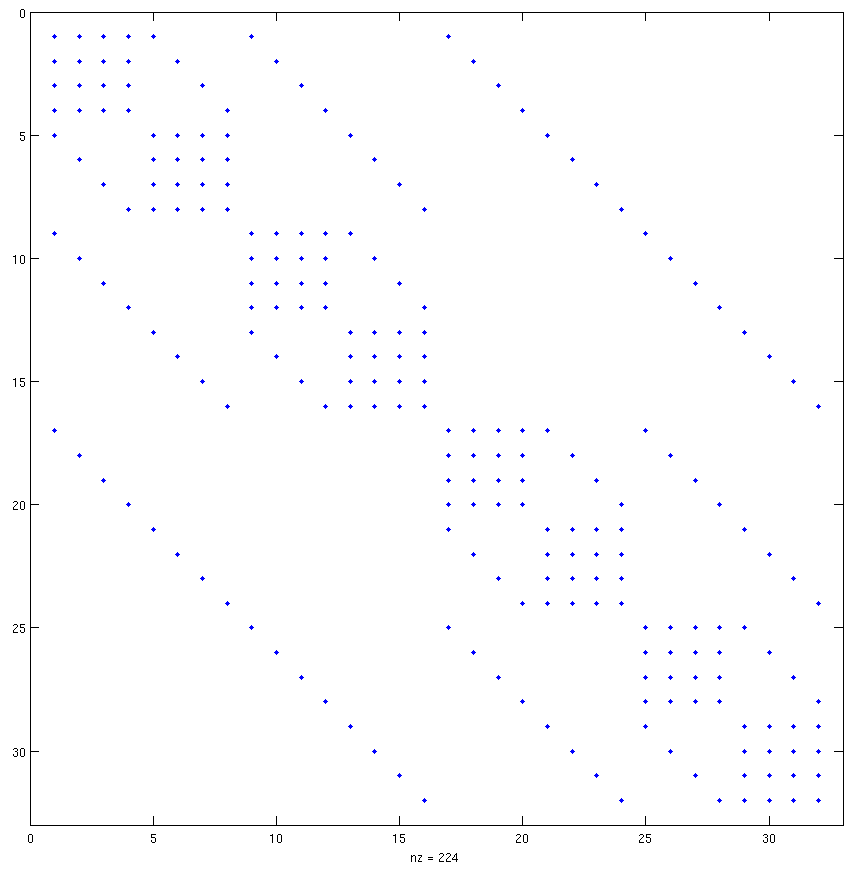
\includegraphics[width=3in]{chapters/spn_equations/group1.png}
  \end{center}
  \caption{\textbf{Sparsity pattern for 1-group $SP_7$
      discretization.} \textit{A $2\times 2 \times 2$ element mesh was
      used to show detail of the blocks formed by the discretization.}}
  \label{fig:group1}
\end{figure}
\begin{figure}[t!]
  \begin{center}
    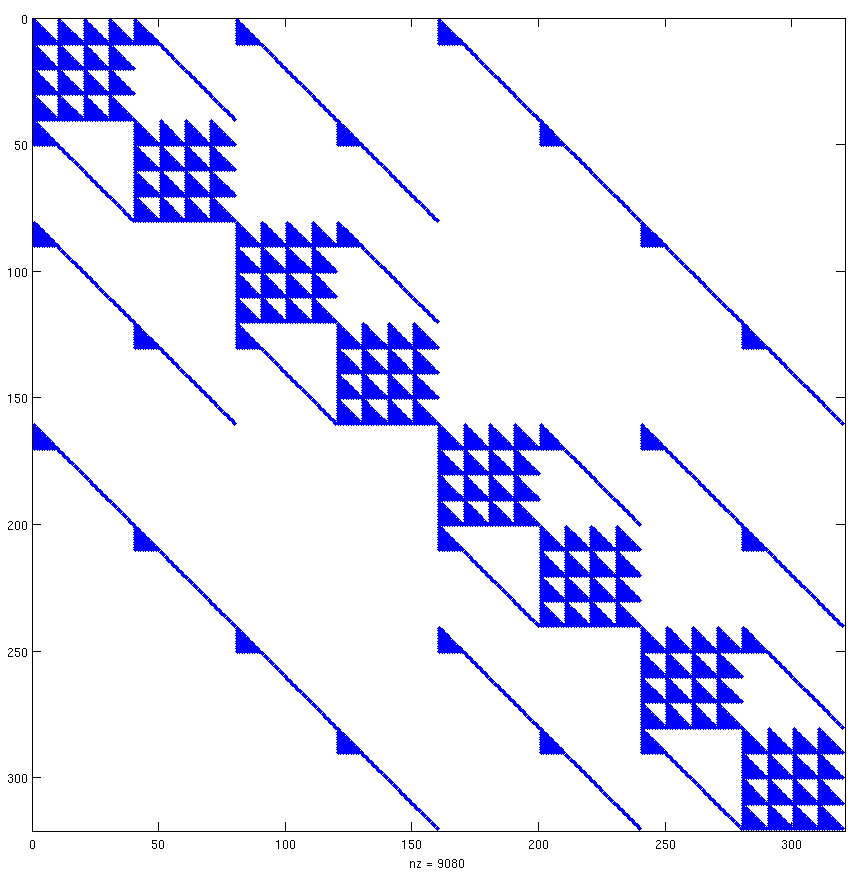
\includegraphics[width=3in]{chapters/spn_equations/group10ds.png}
  \end{center}
  \caption{\textbf{Sparsity pattern for 10-group $SP_7$ discretization
      with downscatter only.} \textit{A $2\times 2 \times 2$ element
      mesh was used to show detail of the blocks formed by the
      discretization.}}
  \label{fig:group10ds}
\end{figure}
\begin{figure}[t!]
  \begin{center}
    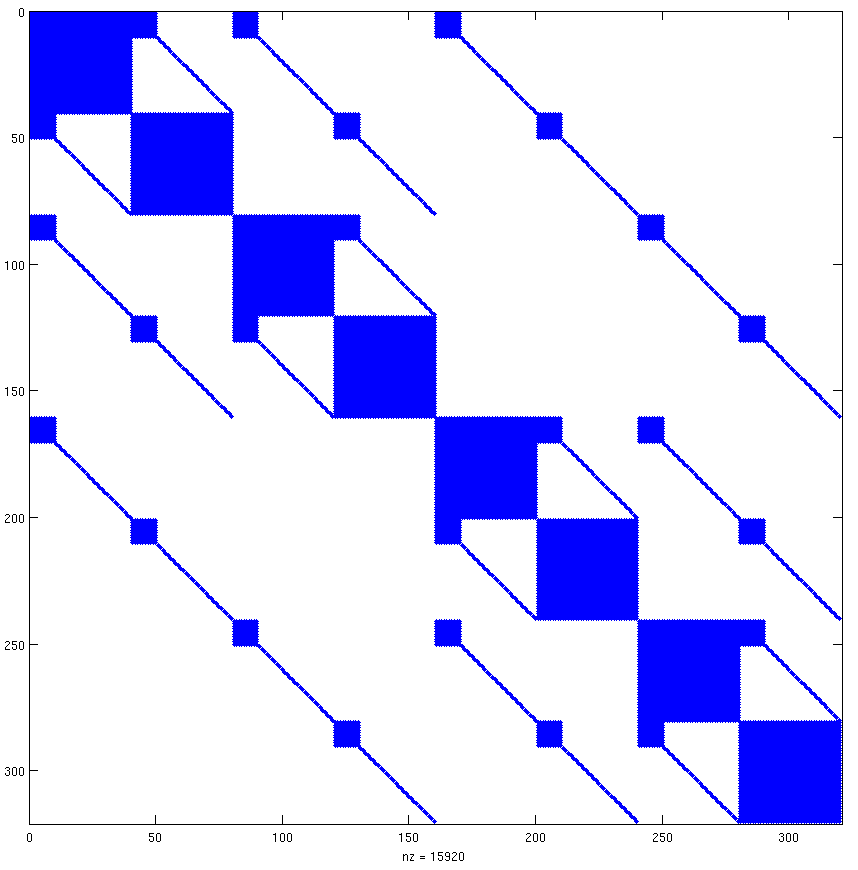
\includegraphics[width=3in]{chapters/spn_equations/group10us.png}
  \end{center}
  \caption{\textbf{Sparsity pattern for 10-group $SP_7$ discretization
      with downscatter and upscatter.} \textit{A $2\times 2 \times 2$ element
      mesh was used to show detail of the blocks formed by the
      discretization.}}
  \label{fig:group10us}
\end{figure}
We note a few key features of the sparsity plots. The first is that
for multigroup problems without full upscatter and downscatter
(i.e. Figure~\ref{fig:group10ds}), the resulting matrix is asymmetric
and therefore a linear solver that can handle asymmetric linear
systems is required. Nearly all problems of interest will not have
full upscattering or downscattering. Second we note the largely
diagonal character of these systems, although the blocks from
Eq~(\ref{eq:A_block_matrix}) are readily apparent. Our first attempt
at preconditioning this system will be to use the point Jacobi
preconditioning from \S\ref{sec:stochastic_preconditioning} due to
this diagonal form.

\subsection{Point Jacobi Spectral Analysis Results}
\label{subsec:spn_analysis_results}
Spectral radius computations were performed for the cases described
above for the point Jacobi preconditioned iteration matrix $\ve{H} =
\ve{I}-\ve{M}^{-1}\ve{A}$ with $\ve{M} =
diag(\ve{A})$. Table~\ref{tab:group1pj} gives the results for the
1-group case, Table~\ref{tab:group10dspj} for the 10-group case with
full downscatter only and Table~\ref{tab:group10uspj} for the 10-group
case with full downscatter and full upscatter.
\begin{table}[t!]
  \begin{center}
    \begin{tabular}{cccccc}\hline\hline
      \multicolumn{1}{c}{}& 
      \multicolumn{1}{c}{}& 
      \multicolumn{1}{c}{}& 
      \multicolumn{1}{c}{$SP_N$ Order}& 
      \multicolumn{1}{c}{}& 
      \multicolumn{1}{c}{} \\
       &   & \textbf{1} & \textbf{3} & \textbf{5} & \textbf{7}  \\
       & \textbf{0} & 0.0635 & 0.6722 & 1.3144 & 1.976 \\
       & \textbf{1} & 0.0666 & 0.6728 & 1.3141 & 1.9755 \\
      $P_N$ Order & \textbf{3} & 0.0666 & 0.6822 & 1.3141 & 1.9755 \\
       & \textbf{5} & 0.0666 & 0.6822 & 1.3278 & 1.9847 \\
       & \textbf{7} & 0.0666 & 0.6822 & 1.3278 & 1.9917 \\
      %%
      \hline\hline
    \end{tabular}
  \end{center}
  \caption{\textbf{Spectral radius results for the point Jacobi
      preconditioned iteration matrix with 1 energy group.}}
  \label{tab:group1pj}
\end{table}
\begin{table}[t!]
  \begin{center}
    \begin{tabular}{cccccc}\hline\hline
      \multicolumn{1}{c}{}& 
      \multicolumn{1}{c}{}& 
      \multicolumn{1}{c}{}& 
      \multicolumn{1}{c}{$SP_N$ Order}& 
      \multicolumn{1}{c}{}& 
      \multicolumn{1}{c}{} \\
       &   & \textbf{1} & \textbf{3} & \textbf{5} & \textbf{7}  \\
       & \textbf{0} & 0.0655 & 0.677 & 1.32 & 1.982 \\
       & \textbf{1} & 0.071 & 0.6777 & 1.319 & 1.982 \\
      $P_N$ Order & \textbf{3} & 0.071 & 0.687 & 1.327 & 1.9872 \\
       & \textbf{5} & 0.071 & 0.687 & 1.336 & 1.997 \\
       & \textbf{7} & 0.071 & 0.687 & 1.336 & 1.9995 \\
      %%
      \hline\hline
    \end{tabular}
  \end{center}
  \caption{\textbf{Spectral radius results for the point Jacobi
      preconditioned iteration matrix with 10 energy groups and full
      downscatter.}}
  \label{tab:group10dspj}
\end{table}
\begin{table}[t!]
  \begin{center}
    \begin{tabular}{cccccc}\hline\hline
      \multicolumn{1}{c}{}& 
      \multicolumn{1}{c}{}& 
      \multicolumn{1}{c}{}& 
      \multicolumn{1}{c}{$SP_N$ Order}& 
      \multicolumn{1}{c}{}& 
      \multicolumn{1}{c}{} \\
       &   & \textbf{1} & \textbf{3} & \textbf{5} & \textbf{7}  \\
       & \textbf{0} & 0.7283 & 0.81 & 1.47 & 2.1446 \\
       & \textbf{1} & 0.7317 & 0.8 & 1.46 & 2.1368 \\
      $P_N$ Order & \textbf{3} & 0.7317 & 0.91 & 1.526 & 2.2274 \\
       & \textbf{5} & 0.7317 & 0.91 & 1.5344 & 2.2562 \\
       & \textbf{7} & 0.7317 & 0.91 & 1.5345 & 2.2842 \\
      %%
      \hline\hline
    \end{tabular}
  \end{center}
  \caption{\textbf{Spectral radius results for the point Jacobi
      preconditioned iteration matrix with 10 energy groups, full
      downscatter and full upscatter.}}
  \label{tab:group10uspj}
\end{table}
It is readily apparent from the tabulated data the point Jacobi
preconditioning is insufficient as a preconditioning mechanism for
problems of order $SP_5$ or higher. In addition, as upscatter is
introduced into the system, a much larger spectral radius is observed
at lower $SP_N$ orders, signaling a need for a better preconditioning
strategy to both ensure and improve covergence for Monte Carlo
methods. 

\subsection{Block Jacobi Preconditioning}
\label{sec:spn_preconditioning}
If Monte Carlo methods are to be used to solve the $SP_N$ system of
equations, a different preconditioning strategy is required in order
to ensure convergence for systems of all $SP_N$ and $P_N$ orders with
arbitrary energy group structures. To achieve this, we look back to
the sparsity plots we generated in Figures~\ref{fig:group1},
\ref{fig:group10ds} and \ref{fig:group10us} as well as the multigroup
$SP_N$ equations. Initially, the diagonal character of the system led
us to try point Jacobi preconditioning with only marginal
results. From the sparsity plots we note the block structure that
ultimately arises from the multigroup scattering matrices and their
insertion into Eq~(\ref{eq:A_block_matrix}). When full upscatter and
downscatter are used the resulting blocks are completely dense while
only downscatter gives a lower triangular scattering matrix and the
block structure shown in Figure~\ref{fig:group10ds}. 

Based on this both block and diagonally dominant structure for
matrices formed by the general multigroup $SP_N$ equations, we instead
choose \textit{block Jacobi} preconditioning as a left preconditioner
for the system. Like point Jacobi preconditioning, block Jacobi
preconditioning extracts the diagonal elements of the matrix as the
preconditioner where now the elements extracted are the blocks on the
diagonal as shown on the left side of
Figure~\ref{fig:block_jacobi_ex}. For the $SP_N$ equations,
Eq~(\ref{eq:A_block_matrix}) gives a block size of $N_g\times(N+1)/2$.
\begin{figure}[t!]
  \begin{center}
    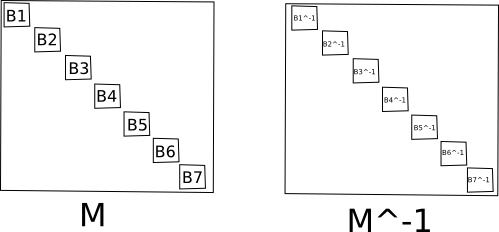
\includegraphics[width=5in]{chapters/spn_equations/block_preconditioning.png}
  \end{center}
  \caption{\textbf{Block Jacobi preconditioning strategy used for the
      $SP_N$ equations.} \textit{Left: The preconditioner is formed by
      the diagonal blocks of the matrix. Right: Inversion is trivial
      and decoupled by block.}}
  \label{fig:block_jacobi_ex}
\end{figure}
The inversion of this preconditioner is trivial as shown on the right
side of Figure~\ref{fig:block_jacobi_ex}. Each block can be inverted
individually and combined to form the inverse. For high performance
implementations this has several attractive properties. First, the
blocks in the matrix come from the energy/angle discretization of the
transport equation as given by Eq~(\ref{eq:A_block_matrix}). Each
block on the diagonal is bound to a mesh element in the system (note
there are 8 blocks on the diagonal in each of the sparsity patterns
with a mesh of $2 \times 2 \times 2$) and therefore we expect the
matrix elements forming the block to be entirely local. Second, these
blocks are typically dense and nearly lower triangular for many
transport problems meaning that established dense matrix methods based
on LU-factorization and other schemes can be used for fast inversion
\citep{lapack_citation}.

\subsection{Block Jacobi Spectral Analysis Results}
\label{subsec:spn_analysis_results}
Spectral radius computations for the block Jacobi preconditioned
iteration matrix were performed for the same problems as the point
Jacobi preconditioned case. Table~\ref{tab:group1bj} gives the results
for the 1-group case, Table~\ref{tab:group10dsbj} for the 10-group
case with full downscatter only and Table~\ref{tab:group10usbj} for
the 10-group case with full downscatter and full upscatter. A block
size of $N_g\times(N+1)/2$ was used for the preconditioner in all
cases.
\begin{table}[t!]
  \begin{center}
    \begin{tabular}{cccccc}\hline\hline
      \multicolumn{1}{c}{}& 
      \multicolumn{1}{c}{}& 
      \multicolumn{1}{c}{}& 
      \multicolumn{1}{c}{$SP_N$ Order}& 
      \multicolumn{1}{c}{}& 
      \multicolumn{1}{c}{} \\
       &   & \textbf{1} & \textbf{3} & \textbf{5} & \textbf{7}  \\
       & \textbf{0} & 0.0635 & 0.1269 & 0.1444 & 0.1513 \\
       & \textbf{1} & 0.0666 & 0.1315 & 0.1474 & 0.1534 \\
      $P_N$ Order & \textbf{3} & 0.0666 & 0.1365 & 0.154 & 0.1592 \\
       & \textbf{5} & 0.0666 & 0.1365 & 0.1562 & 0.163 \\
       & \textbf{7} & 0.0666 & 0.1365 & 0.1562 & 0.164 \\
      %%
      \hline\hline
    \end{tabular}
  \end{center}
  \caption{\textbf{Spectral radius results for the block Jacobi
      preconditioned iteration matrix with 1 energy group.}}
  \label{tab:group1bj}
\end{table}
\begin{table}[t!]
  \begin{center}
    \begin{tabular}{cccccc}\hline\hline
      \multicolumn{1}{c}{}& 
      \multicolumn{1}{c}{}& 
      \multicolumn{1}{c}{}& 
      \multicolumn{1}{c}{$SP_N$ Order}& 
      \multicolumn{1}{c}{}& 
      \multicolumn{1}{c}{} \\
       &   & \textbf{1} & \textbf{3} & \textbf{5} & \textbf{7}  \\
       & \textbf{0} & 0.0647 & 0.1275 & 0.1449 & 0.1514 \\
       & \textbf{1} & 0.0686 & 0.1338 & 0.1484 & 0.1547 \\
      $P_N$ Order & \textbf{3} & 0.0687 & 0.1399 & 0.1582 & 0.1625 \\
       & \textbf{5} & 0.0692 & 0.1399 & 0.1582 & 0.1657 \\
       & \textbf{7} & 0.0678 & 0.1393 & 0.1624 & 0.166 \\
      %%
      \hline\hline
    \end{tabular}
  \end{center}
  \caption{\textbf{Spectral radius results for the block Jacobi
      preconditioned iteration matrix with 10 energy groups and full
      downscatter.}}
  \label{tab:group10dsbj}
\end{table}
\begin{table}[t!]
  \begin{center}
    \begin{tabular}{cccccc}\hline\hline
      \multicolumn{1}{c}{}& 
      \multicolumn{1}{c}{}& 
      \multicolumn{1}{c}{}& 
      \multicolumn{1}{c}{$SP_N$ Order}& 
      \multicolumn{1}{c}{}& 
      \multicolumn{1}{c}{} \\
       &   & \textbf{1} & \textbf{3} & \textbf{5} & \textbf{7}  \\
       & \textbf{0} & 0.1887 & 0.2267 & 0.2285 & 0.2286 \\
       & \textbf{1} & 0.4535 & 0.5044 & 0.5045 & 0.5045 \\
      $P_N$ Order & \textbf{3} & 0.4535 & 0.6453 & 0.6506 & 0.6506 \\
       & \textbf{5} & 0.4535 & 0.6453 & 0.6802 & 0.6818 \\
       & \textbf{7} & 0.4535 & 0.6453 & 0.6802 & 0.6927 \\
      %%
      \hline\hline
    \end{tabular}
  \end{center}
  \caption{\textbf{Spectral radius results for the block Jacobi
      preconditioned iteration matrix with 10 energy groups, full
      downscatter and full upscatter.}}
  \label{tab:group10usbj}
\end{table}
From the tabulated block Jacobi data it is clear that this is the
preferred preconditioning choice for all $SP_N$ problems in term of
Monte Carlo solution methods. All cases were observed to have a
spectral radius below unity and often significantly smaller than that,
greatly improving convergence rates over the point Jacobi preconditioned
problem.

%%---------------------------------------------------------------------------%%
\section{Fuel Assembly Criticality Calculations}
\label{sec:fuel_assembly_calcs}

\subsection{Jacobi Preconditioned Calculations}
\label{subsec:jacobi_prec_assembly_calc}

\subsection{MCSA Break Down}
\label{subsec:mcsa_break_down}

\subsection{Advanced Preconditioning Strategies}
\label{subsec:spn_advanced_preconditioning}

\subsubsection{ILUT Preconditioning}
\label{subsubsec:spn_ilut_preconditioning}

\subsubsection{Sparse Approximate Inverse Preconditioning}
\label{subsubsec:spn_spainv_preconditioning}

\subsubsection{SPAINV Improved ILUT Preconditioning}
\label{subsubsec:spn_spainv_preconditioning}

\subsection{MCSA Comparison to Conventional Methods}
\label{subsec:spn_comparison}
